\clearpage
\section{Definition of three major types of construtors for the SiconosmodelXML objects.}


\subsection{Default constructor}

\begin{verbatim}
ObjectXML::ObjectXML() 
{

}
\end{verbatim}
%\ac{tbd}



\subsection{Constructor from an XML node}


\begin{verbatim}


ObjectXML::ObjectXML( xmlNode* rootNodeOfTheObjectXML ) 
{

}
\end{verbatim}
%\ac{tbd}
\clearpage
\section{Detailed implementation of the Model Loading : Unfolding of the creation of the platform}
The two ways to construct the platform are using similar mechanisms, and especially the same creating
method.



\subsection{Model loading form an XML file}


At first, when a XML file is loaded, the data of the file are copied in memory in a DOM tree. From
there, the XML Management platform is built.\\
The SiconosModelXML owns the DOM tree and create NSDSXML and StrategyXML objects. The created objects
only know the branch of the DOM tree relating to them. Gradually, the NSDSXML will create the
different XML objects of the dynamical systems (DSXML, LagrangianNLDSXML, LagrangianTIDSXML,
LinearSystemDSXML), and the different interactions.\\
Then, after all the XML objects have been created, the \ac{siconos} platform is built.\\
The Model which has lead the construction of the XML platform begin the creation of the NSDS,
DynamicalSystem, LagrangianNLDS, ..., Interaction, Relation, ..., NonSmoothLaw, ..., Strategy,
TimeDiscretisation, OneStepIntegrator, Moreau, ..., OneStepNSProblem, LCP and QP by using the
relating XML objects.\\
The construction of each object of the platform is made by calling a
"createXxxxx" method (createModel(...), createNSDS(...), createStrategy(...), ...). One parameter
corresponding to the XML object is enough to give the right data to the platform's object for his
construction.


\begin{figure}
\begin{center}
        \includegraphics[scale=0.75, clip]{figure/platform_loading_XML.ps}
        \caption{Sequence diagram of the platform's loading with XML file}
        \label{fig: platform's loading1}
\end{center}
\end{figure}

The "create"methods used are partially shown in the diagram \ref{fig: platform's loading1}.







\subsection{Creating a model through the API C++}


The construction of the platform we can see in the diagram \ref{fig: platform's loading2} is lead by an user. The user calls a constructor of the object that he want to create and after that adds the object to the SiconosModel of necessary. For instance, the sequence in the listing \ref{Lst:Creating} can be invoked for creating a model with a DynamicalSystem of the type LagrangianLinearTIDS.

\begin{lstlisting}[frame=single, caption={Creating a model through the API C++,label={Lst:Creating}}]
  // Default Constructor of a Model
  Model model1; 
  // Constructor of a nsds with minimal data 
  NonSmoothDynamicalSystem nsds1( false );
  // Set the NonSmoothDynamicalSystem of the Model
  model1.setNonSmoothDynamicalSystem(nsds1) ;
        
  SimpleVector q0(3);
  q0.zero();  q0(0) = 1.0;                
  SimpleVector v0(3);
  v0.zero();             
  SiconosMatrix mass(3, 3);
  mass.eye();
  SiconosMatrix K(3, 3);
  K.zero();                
  SiconosMatrix C(3, 3);
  C.zero();

  // Constructor of a LagrangianLinearTIDS with minimal data 
  LagrangianLinearTIDS lltids1(1, 3, &q0, &v0, &mass,
                               "BasicPlugin:FExt",&K, &C);

  nsds1.addDS(&lltids1);

\end{lstlisting}





 Due to the fact that the destructor of the nsds delete actually the DynamicalSystem which are contained in it, we need to declare a pointer on a DS in  order to avois a doucle delete at the end of the run, see Listing \ref{Lst:Creatingbis}

\begin{lstlisting}[frame=single, caption={Creating a model through the API C++, bis},label={Lst:Creatingbis}]
  LagrangianLinearTIDS *lltids1;
  // Constructor of a LagrangianLinearTIDS with minimal data 
  lltids1 = new LagrangianLinearTIDS(1, 3, &q0, &v0, &mass,
                                     "BasicPlugin:FExt",&K, &C);
  nsds1.addDS(lltids1);
\end{lstlisting}
\begin{ndr}
We need to define precisely a rule for the constructor/destructor with new/delete
\end{ndr}
In the same way,  a complete model may be constructed using the specific constructor of each object. After this operation, we can use either the member function \texttt{setAttributeObject} for pointing or  a member function  \texttt{addAttributeObject} in the case of a vector attribute

 Here are a non exhaustive list of such methods

 \begin{itemize}
 \item In the Model class :
\begin{verbatim}
Model::Model();
Model::setNSDS(NonSmoothDynamicalSystem nsds)
Model::setStrategy(Strategy s)
\end{verbatim}
 \item In the NonSmoothDynamicalSystem class :
\begin{verbatim}
NonSmoothDynamicalSystem::NonSmoothDynamicalSystem(bool BVP)
NonSmoothDynamicalSystem::addDS(DynamicalSystem ds1) // push_back in the vector of pointer on DS
NonSmoothDynamicalSystem::addInteraction(Interaction in1) 
\end{verbatim}  
 \item In the DynamicalSystem class :
\begin{verbatim}
DynamicalSystem::DynamicalSystem(number, n, x0, BasicPlugin:vectorField)
DynamicalSystem::setBC()
\end{verbatim}
 \item In derived class of DynamicalSystem :
\begin{verbatim}
LinearDS::LinearDS(number, n, x0, A)
LagrangianDS::LagrangianDS(number, ndof, q0, velocity0, BasicPlugin:computeMass,
                BasicPlugin:computeFInt, BasicPlugin:computeFExt,
                BasicPlugin:computeJacobianQFInt, BasicPlugin:computeJacobianVelocityFInt,
                BasicPlugin:computeJacobianQQNLInertia,
                BasicPlugin:computeJacobianVelocityQNLInertia, BasicPlugin:computeQNLInertia)
LagrangianLinearTIDS::LagrangianLinearTIDS(number, ndof, q0, velocity0, BasicPlugin:computeMass, BasicPlugin:computeFExt, K, C)
\end{verbatim}

   
          \item In the Interaction class :
\begin{verbatim}
Interaction::Interaction(number)
addDS(DynamicalSystem * dsi )
setRelation(Relation r)
setNSLaw(Relation r)
\end{verbatim}
          \item In the Relation class :
\begin{verbatim}
Relation::Relation(number,BasicPlugin:computeInput,,BasicPlugin:computeOutput)
\end{verbatim}
          \item In the NSLaw class :
\begin{verbatim}
NSLaw::NSLaw()
\end{verbatim}
 \item In the Strategy class :
\begin{verbatim}
 Strategy::Strategy()
 setTimeDiscretisation(TimeDiscretisation td)
 addOneStepIntegrator(OneStepIntegrator osi) 
\end{verbatim}    
\item ....
 \end{itemize}




%%  The unfolding of the building of the platform's architecture is described in the next sequence diagram.
%% \begin{figure}
%% \begin{center}
%%         \includegraphics[scale=0.75, clip]{figure/platform_loading.ps}
%%         \caption{Sequence diagram of the platform's loading without XML file}
%%         \label{fig: platform's loading2}
%% \end{center}
%% \end{figure}


\subsection{Mixed strategies}
This means that the data read in the file are supplemented with information given in the command
program.
In this case, the XML file is similar to the previous case, then the way to create objects of
the platform apart from a XML file will be detailed in the next section.






